% ---
% type: Article
% title: LaTeX Reference Project
% authors:
%   - type: Person
%     givenNames:
%       - Karl
%       - R
%     familyNames: Popper
%     affiliation:
%       type: University
%       name: University of Canterbury
%       address:
%         type: PostalAddress
%         addressCountry: New Zealand
%         addressLocality: Christchurch
%   - type: Person
%     givenNames: Auguste
%     familyNames: Comte
%     affiliation:
%       - type: Organization
%         name: University of Montpellier
%         url: www.umontpellier.fr/en
%         address:
%           type: PostalAddress
%           addressCountry: France
%           addressLocality: Montpellier
%       - type: Organization
%         name: École Polytechnique      
%         address:
%           type: PostalAddress
%           addressCountry: France
%           addressLocality: Paris
%   - type: Person
%     givenNames: Francis
%     familyNames: Bacon
%     affiliation:
%       - type: Organization
%        name: Trinity College
%        address:
%          type: PostalAddress
%          addressCountry: United Kingdom
%          addressLocality: Cambridge
%        parentOrganization:
%          type: Organization
%          name: University of Cambridge
% bibliography: refs.bib
% ---



\documentclass[12pt]{article}

% --- Packages --- %

\usepackage{authblk} % for marking up authorship; \affil{} command (and customizations)
\usepackage{hyperref} % for hyperlinks; \href{} command
\usepackage{setspace} % for line spacing; \onehalfspacing command
\usepackage{listings} % for lstlisting environment
\usepackage{minted} % for YAML environment
\usepackage{xcolor} % for defining colors
\usepackage{graphicx}

% --- Customization --- %

\renewcommand\Affilfont{\fontsize{10}{11}\itshape} % font size of affil

% remove * from thanks
\makeatletter
\def\thanks#1{\protected@xdef\@thanks{\@thanks
        \protect\footnotetext{#1}}}
\makeatother

% custom Python listing environment
\definecolor{codegreen}{rgb}{0,0.6,0}
\definecolor{codegray}{rgb}{0.5,0.5,0.5}
\definecolor{codepurple}{rgb}{0.58,0,0.82}
\lstdefinestyle{pythoncustomstyle}{  
commentstyle=\color{codegreen},
keywordstyle=\color{magenta},
numberstyle=\tiny\color{codegray},
stringstyle=\color{codepurple},
basicstyle=\ttfamily\footnotesize,
breakatwhitespace=false,         
breaklines=true,                 
captionpos=b,                    
keepspaces=true,                 
numbers=left,                    
numbersep=5pt,                  
showspaces=false,                
showstringspaces=false,
showtabs=false,                  
tabsize=4,
frame=single
}
    
% --- Content --- %

\begin{document}

\onehalfspacing

\title{LaTeX Reference Project}

\author[1]{Karl R. Popper\textsuperscript{*}\thanks{*Authors contributed equally to this study; karl@poppermail.com, comte@astuteauguste.com}}
\author[2,3]{Auguste Comte\textsuperscript{*}}
\author[4]{Francis Bacon}

\affil[1]{University of Canterbury, Christchurch, New Zealand}
\affil[2]{University of Montpellier, Montpellier, France}
\affil[3]{\'{E}cole Polytechnique, Paris, France}
\affil[4]{Trinity College, University of Cambridge, Cambridge, United Kingdom}

\maketitle

\begin{abstract}
In the abstract you will summarize the motivation, results and
conclusions of the manuscript.
The abstract is the most read section of the entire paper, so 
making it concise, precise and punchy is critical.
Sometimes authors write in the present tense, sometimes in the past
tense -- it is more a matter of style.

\end{abstract}

\clearpage

\section*{Introduction}

The present document is meant to help you set up a \LaTeX
(\texttt{.tex}) manuscript to be converted into any format supported by
Stencila.
It has been written by a scientist for scientists; of course, not
everything you can do with \LaTeX  will have found its way into this
tutorial.
If you \textbf{really} need support for some obscure \LaTeX
functionality that Stencila does not already cover, you can make a
pull request (PR) on one of our repositories, like Encoda's
(\href{Encoda repo}{https://stenci.la/encoda}).

\subsection*{YAML commented block at the top}
The attentive reader will have noticed that at the top of this
\texttt{.tex} file, there are many commented lines with \texttt{\%}
containing YAML code:

{\singlespace
\begin{minted}[gobble=0,frame=single,linenos]{yaml}
type: Article
title: LaTeX Reference Project
authors:
  - type: Person
    givenNames:
      - Karl
      - R
    familyNames: Popper
    affiliation:
      type: University
      name: University of Canterbury
      address:
        type: PostalAddress
        addressCountry: New Zealand
        addressLocality: Christchurch
  - type: Person
    givenNames: Auguste
    familyNames: Comte
    affiliation:
      - type: Organization
        name: University of Montpellier
        url: www.umontpellier.fr/en
        address:
          type: PostalAddress
          addressCountry: France
          addressLocality: Montpellier
      - type: Organization
        name: École Polytechnique      
        address:
          type: PostalAddress
          addressCountry: France
          addressLocality: Paris
  - type: Person
    givenNames: Francis
    familyNames: Bacon
    affiliation:
      - type: Organization
       name: Trinity College
       address:
         type: PostalAddress
         addressCountry: United Kingdom
         addressLocality: Cambridge
       parentOrganization:
         type: Organization
         name: University of Cambridge
\end{minted}
}

\noindent (The box above was rendered with the \LaTeX 's \texttt{minted}
package.)

This commented YAML block needs to be at the top of the file so that
Stencila's internal programs can first parse and then reformat the
article's metadata.

\section*{Methods}

In the Methods section we often find equations like this:

\begin{equation}
  f(x) = \frac{1}{\sigma
    \sqrt{2\pi}}e^{\frac{1}{2}(\frac{x-\mu}{\sigma})}.
  \label{eq:normal}
\end{equation}

Equation \ref{eq:normal} is the probability density function of a
normal distribution.
But math can also appear inline: $x \sim \mathcal{N}(\mu,
\sigma^2)$.

\section*{Results}

In the Results section you will likely want to add some figures,
tables, static and executable code chunks, to name a few.

\subsection*{Regular figures and tables}

It is easy to place different kinds of figures.
You can, for example, decorate your manuscript with a photo of the
best animal out there: the panda bear.

\begin{figure}
  \centering
  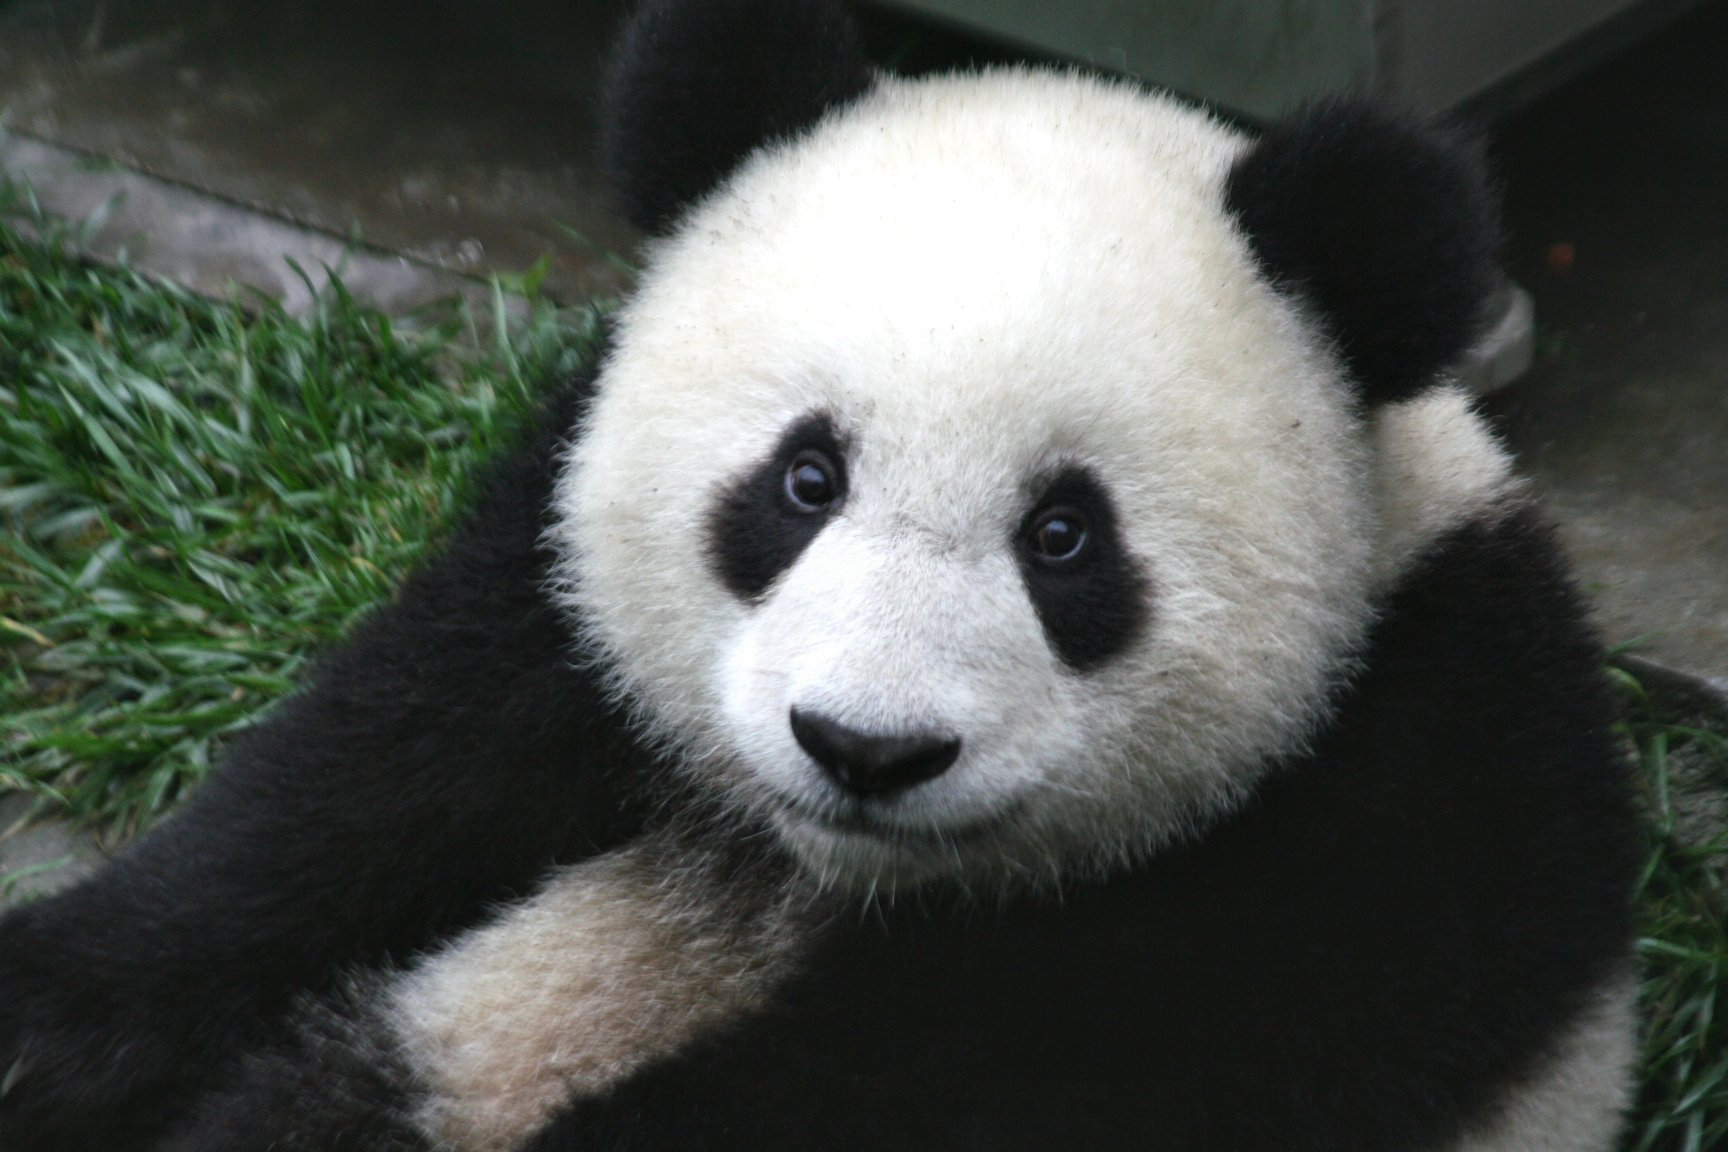
\includegraphics[width=12cm]{figs/pandacub.jpeg}
  \caption{The most adorable animal, hands down.}
  \label{fig:panda}
\end{figure}  

As you know, you can refer back to Fig. \ref{fig:panda}.

Of course, we can also introduce tables, and refer back to them: Table
\ref{tab:playerscores}.

\begin{table}[h!]
  \centering
  \begin{tabular}{ c c }
    \hline
    Name & Score\\
    \hline
    KP & 10\\
    Gus & 11\\
    Bacon & 7\\
    \hline
  \end{tabular}
  \caption{Player scores.}
  \label{tab:playerscores}
\end{table}

\subsection*{Code chunks}

Code chunks play an important role in live, reproducible articles.
It is through code chunks that authors (i) specify how to build the
figures they want to show, and (ii) execute arbitrary computations
required for generating results.
The main difference between code chunks and static code blocks (e.g.,
the YAML block above) is that code chunks are executable.
Code chunks are specified by adding \texttt{\% begin exec} right
before the code block, and \texttt{\% end exec} right after.
(In \LaTeX, these short strings will not appear in the
compiled document.)

\subsubsection*{Python code chunks}

The following code chunk is written in Python and
executed by the Stencila engine:\\

\noindent \texttt{\% begin exec}
% begin exec
\begin{lstlisting}[language=Python, style=pythoncustomstyle,
  caption={Customizing some aspects of plotting before it is actually
    done.}]
import numpy as np
import matplotlib.pyplot as plt

plt.rcParams.update({
    "text.usetex": True,
    "font.family": "serif",
    "font.serif": ["Palatino"],
})
\end{lstlisting}
\noindent \texttt{\% end exec}\\
% end exec

Note that the Python code above is not only executed, but the state of
variables is saved and conserved for future Python code chunks.
For example, if we now add another code chunk, it inherits whatever
was executed previously:\\

\noindent \texttt{\% begin exec}
% begin exec
\begin{lstlisting}[language=Python, style=pythoncustomstyle,
  caption={Histogram of 1,000 random draws from $\mathcal{N}$(0.0, 1.0).}]
mu = 0.0
sigma = 1.0
x = mu + sigma * np.random.randn(1000)
% end exec
\noindent  \texttt{\% end exec}

num_bins = 30
fig = plt.figure()
ax = fig.add_subplot(1,1,1)
ax.hist(x, num_bins, facecolor='gray', alpha=0.5)
ax.set_xlabel('Random variable $x$')
ax.set_ylabel('Frequency')
ax.spines['top'].set_visible(False)
ax.spines['right'].set_visible(False)
plt.title(r'Histogram of 1,000 draws from $\mathcal{N}$(0.0, 1.0):')
plt.show()
\end{lstlisting}
\noindent \texttt{\% end exec}\\
% end exec

The above code chunk should be rendered into a histogram plot (note
how Python libraries were actually loaded in the previous code chunk
window!).
Alternatively, you can just point the code chunk environment to a
Python script, e.g., `pythonstuff/pythonscatter.py':\\

\noindent \texttt{\% begin exec}
% begin exec
\lstinputlisting[language=Python, style=pythoncustomstyle,
  caption={Scatterplot of 1,000 random draws from $\mathcal{N}$(0.0, 1.0) as
    a function of their indices.}]{pythonstuff/pythonscatter.py}
\noindent \texttt{\% end exec}\\
% end exec

\subsubsection*{R code chunks}

The following code chunk is written in R and
executed by the Stencila engine:\\

\noindent \texttt{\% begin exec}
% begin exec
\begin{lstlisting}[language=R, breaklines=true, showspaces=false,
  showstringspaces=false, tabsize=4, captionpos=b, frame=single,
  caption={Histogram of 1,000 random draws from $\mathcal{N}$(0.0, 1.0).}]
library(ggplot2)
  
x = rnorm(1000)

ggplot(data.frame(x), aes(x=x)) + geom_histogram(fill="lightgray", color=NA) + theme_classic() + xlab("Random variable x") + ylab("Frequency")
\end{lstlisting}
% end exec
\noindent  \texttt{\% end exec}

\end{document}

% On Emacs, C-x C-n to evaluate the following before compiling
%%% Local Variables:
%%% LaTeX-command: "latex -shell-escape"
%%% End: